
\documentclass[xcolor=pdftex,table,11pt]{beamer}
\usetheme{Warsaw}
\usepackage[utf8]{inputenc}
\usepackage[english]{babel}
\usepackage{amsmath}
\usepackage{amsfonts}
\usepackage{amssymb}
\usepackage{multirow}
\usepackage{siunitx}
\usepackage{listings}
\usepackage{tabulary}
\usepackage[highlightcolor=yellow]{../styles/code}
\author{Informática I - Instituto Unviersitario Areonáutico}
\title{Introducción a los algoritmos}

\usepackage{booktabs}
\usepackage{longtable}
\newcommand*{\thead}[1]{\multicolumn{1}{c}{\bfseries #1}}


%\setbeamercovered{transparent} 
%\setbeamertemplate{navigation symbols}{} 
%\logo{} 
%\institute{} 
%\date{} 
%\subject{} 
\begin{document}


\begin{frame}
\titlepage
\end{frame}

\begin{frame}
\tableofcontents
\end{frame}

\begin{frame}{¿Qué son los algoritmos?}
\begin{block}{Según la RAE}
         Conjunto ordenado y finito de operaciones que permite hallar la solución a un problema.
    \end{block}
 
 \begin{block}{Según Deitel}
         Es el procedimiento para resolver un problema en términos de las acciones a ejecutar y el órden en el cual se llevan a cabo dichas acciones.
    \end{block}
    
\begin{block}{¿Cómo está compuesto un algoritmo?}
   \begin{itemize}
   \item Entrada
   \item Procesamiento
   \item Salida
   \end{itemize}
\end{block}


\end{frame}



\begin{frame}{Ejemplos de algoritmos}

\begin{block}{Preparar una taza de té}
   \begin{itemize}
   \item Entrada: agua, saquito de té, taza
   \item Salida: té caliente
   \item Procedimiento: 
   \begin{itemize}
   \item[]<1-> Inicio del algoritmo

   \begin{itemize}
   
     	\item<1-> Poner el agua fría dentro de la pava
     	 \item<2-> Encender el fuego 
     	 \item<3-> Poner la pava sobre el fuego
   		\item<4-> Esperar que el agua se caliente
   		\item<5-> Poner el saquito de té en la taza
 		\item<6-> Agregar el agua caliente
 		\item<7-> Apagar el fuego
 		\item<8-> Esperar un minuto
 		
   \end{itemize}
 \item[]<9-> Fin del algoritmo

	\end{itemize}
\end{itemize}

\end{block}


\end{frame}



\begin{frame}{Ejemplo de algoritmos}

\begin{block}{Calcular la distancia recorrida por un móvil que se movió en MRUV}
    \begin{equation}\label{eq:d_mruv}
            x(t) = V_0 t + \frac{1}{2}  a  t^2  
    \end{equation}
   \begin{itemize}
   \item Entrada: velocidad inicial, tiempo recorrido, aceleración
   \item Salida: distancia recorrida
   \item Procedimiento: 
   \begin{itemize}
   \item[]<1-> Inicio del algoritmo

   \begin{itemize}
   
     	\item<1-> Ingresar la velocidad inicial del movil
        \item<2-> Ingresar el tiempo de desplazamiento
 		\item<3-> Ingresar la aceleración
 		\item<4-> Aplicar la fórmula \ref{eq:d_mruv}
 		\item<5-> Informar la distancia
   \end{itemize}
 \item[]<6-> Fin del algoritmo

	\end{itemize}
\end{itemize}

\end{block}


\end{frame}



\begin{frame}{Pseudocódigo}
\begin{block}{Definición}

El pseudocódigo es un lenguaje artificial e informal que ayuda a los programadores a desarrollar y probar algoritmos.
\end{block}
\begin{block}{Ejemplo para calcular el volumen de una esfera}

 \begin{itemize}
   \item[]<1-> Inicio del algoritmo

   \begin{itemize}
   
     	\item<1-> Imprimir: Ingrese el radio de la esfera
        \item<2-> Leer: radio
 		\item<3-> $v_{esfera} =\frac{4}{3}  \pi  r^3  $
 		\item<4-> Imprimir: "El volumen de la esfera es $v_{esfera}$"
   \end{itemize}
 \item[]<5-> Fin del algoritmo

	\end{itemize}
\end{block}


\end{frame}

\begin{frame}{Diagrama de flujo}
\begin{columns}
\column{0.5\textwidth}
 \begin{itemize}
   
     	\item<1-> Es la representación gráfica de un algoritmo
        \item<2-> Se dibujan mediante símbolos de propósito especial: rectángulos, rombos, olvalos y círculos entre otros
 		\item<3-> Estos símbolos se conectan mediantes flechas llamadas \textbf{líneas de flujo}
 		\item<4-> \textbf{Tienen un solo punto de inicio y fin}.
   \end{itemize}
\column{0.5\textwidth}
 \begin{figure}
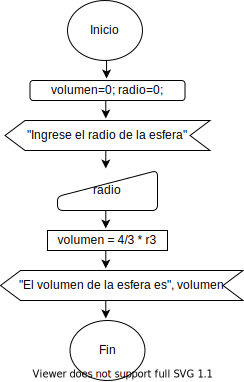
\includegraphics[scale=0.4]{../img/exported/volumen_esfera.png}
\caption{Diagrama de flujo para el cálculo del volúmen de una esfera}
\end{figure}
\end{columns}
\end{frame}






\end{document}